\section{Experiments}  \label{Experiments}

In this section, we first present a comparative analysis of the proposed model on the video object detection task. Second, we present an ablation study analyzing the effects of different training procedures on the robustness of the model to sensor failure scenarios.

\subsection{Training for Bounding Boxes} \label{Experiments:TrainingBoundingBoxes}

We train the RPerceiver with used AdamW optimizer \cite{loshchilovDecoupledWeightDecay2019a} setting the initial learning rates for the movel $ 10^{-4} $. We trained for 31 epochs with a learning rate drop by a factor of 10 at epoch 18 and 28. Data augmentation pipeline includes normalization based on pre-calculated dataset statistics, and frames are resized to a fixed dimension 320 x 320 \cite{redmonYOLO9000BetterFaster2016}. Other training hyperparameters can be found in section \ref{Appendix:TrainingHyperparameters}.

\subsection{Comparison Analysis} \label{Experiments:ComparisonAnalysis}

First, we consider the task of object detection using the detection-moving-mnist-easy benchmark from Section \ref{Methods:Dataset}. We perform a comparative analysis against a still-image object detector of comparable size, YOLOv8n \cite{Jocher_Ultralytics_YOLO_2023}. The primary goal is to evaluate how the proposed RPerceiver architecture utilizes spatio-temporal information from the video input. Results are shown in Table \ref{tab:model_comparison}.

% YOLO: Raw mAP Results (Evaluator): {'map': tensor(0.9231), 'map_50': tensor(0.9621), 'map_75': tensor(0.9410), 'map_small': tensor(0.9231), 'map_medium': tensor(-1.), 'map_large': tensor(-1.), 'mar_1': tensor(0.7471), 'mar_10': tensor(0.9393), 'mar_100': tensor(0.9393), 'mar_small': tensor(0.9393), 'mar_medium': tensor(-1.), 'mar_large': tensor(-1.), 'map_per_class': tensor(-1.), 'mar_100_per_class': tensor(-1.), 'classes': tensor([0, 1, 2, 3, 4, 5, 6, 7, 8, 9], dtype=torch.int32)}

% RPerceiver: Raw mAP Results (Evaluator): {'map': tensor(0.9025), 'map_50': tensor(0.9688), 'map_75': tensor(0.9442), 'map_small': tensor(0.9025), 'map_medium': tensor(-1.), 'map_large': tensor(-1.), 'mar_1': tensor(0.7367), 'mar_10': tensor(0.9240), 'mar_100': tensor(0.9240), 'mar_small': tensor(0.9240), 'mar_medium': tensor(-1.), 'mar_large': tensor(-1.), 'map_per_class': tensor(-1.), 'mar_100_per_class': tensor(-1.), 'classes': tensor([0, 1, 2, 3, 4, 5, 6, 7, 8, 9], dtype=torch.int32)}

% TODO: recompute GFLOPS

\begin{table}[htb!]
    \centering
    \caption{Comparison with the baseline still image detector YOLOv8n \cite{Jocher_Ultralytics_YOLO_2023} on the detection-moving-mnist-easy test split. 'Post' indicates the use of postprocessing heuristics. RPerceiver achieves slightly better $mAP_{50}$ and $mAP_{75}$, but shows worse $mAP_{50-95}$ results. However, RPerceiver achieves these results with significantly fewer parameters and lower computational cost.}
    \label{tab:model_comparison}
    \begin{tblr}{width=1\textwidth, hlines, vlines,
                  colspec = { l c c c c c },
                  row{1} = {font=\bfseries},
                 }
        Model      & Post & mAP_{50} & mAP_{75} & mAP_{50-95} & Params (M)   & GFLOPS         \\
        YOLOv8n    & X & 96.2  & 94.1 & \textbf{92.3}  & 3            & 8.1            \\
        RPerceiver & X & \textbf{96.9} & \textbf{94.4} & 90.3 &\textbf{1} & \textbf{1.2}   \\
    \end{tblr}
\end{table}

% YOLO:
% Raw Overlap mAP Results (Evaluator): {'map': tensor(0.8266), 'map_50': tensor(0.9133), 'map_75': tensor(0.8788), 'map_small': tensor(0.8266), 'map_medium': tensor(-1.), 'map_large': tensor(-1.), 'mar_1': tensor(0.7744), 'mar_10': tensor(0.8536), 'mar_100': tensor(0.8536), 'mar_small': tensor(0.8536), 'mar_medium': tensor(-1.), 'mar_large': tensor(-1.), 'map_per_class': tensor(-1.), 'mar_100_per_class': tensor(-1.), 'classes': tensor([0, 1, 2, 3, 4, 5, 6, 7, 8, 9], dtype=torch.int32)}

% Raw Boundary mAP Results (Evaluator): {'map': tensor(0.6989), 'map_50': tensor(0.7667), 'map_75': tensor(0.7365), 'map_small': tensor(0.6989), 'map_medium': tensor(-1.), 'map_large': tensor(-1.), 'mar_1': tensor(0.7119), 'mar_10': tensor(0.7280), 'mar_100': tensor(0.7280), 'mar_small': tensor(0.7280), 'mar_medium': tensor(-1.), 'mar_large': tensor(-1.), 'map_per_class': tensor(-1.), 'mar_100_per_class': tensor(-1.), 'classes': tensor([0, 1, 2, 3, 4, 5, 6, 7, 8, 9], dtype=torch.int32)}

% RPerceiver
% Raw Overlap mAP Results (Evaluator): {'map': tensor(0.6940), 'map_50': tensor(0.8853), 'map_75': tensor(0.7777), 'map_small': tensor(0.6940), 'map_medium': tensor(-1.), 'map_large': tensor(-1.), 'mar_1': tensor(0.6686), 'mar_10': tensor(0.7389), 'mar_100': tensor(0.7389), 'mar_small': tensor(0.7389), 'mar_medium': tensor(-1.), 'mar_large': tensor(-1.), 'map_per_class': tensor(-1.), 'mar_100_per_class': tensor(-1.), 'classes': tensor([0, 1, 2, 3, 4, 5, 6, 7, 8, 9], dtype=torch.int32)}

% Raw Boundary mAP Results (Evaluator): {'map': tensor(0.8470), 'map_50': tensor(0.9552), 'map_75': tensor(0.9101), 'map_small': tensor(0.8470), 'map_medium': tensor(-1.), 'map_large': tensor(-1.), 'mar_1': tensor(0.8512), 'mar_10': tensor(0.8739), 'mar_100': tensor(0.8739), 'mar_small': tensor(0.8739), 'mar_medium': tensor(-1.), 'mar_large': tensor(-1.), 'map_per_class': tensor(-1.), 'mar_100_per_class': tensor(-1.), 'classes': tensor([0, 1, 2, 3, 4, 5, 6, 7, 8, 9], dtype=torch.int32)}

% TODO: complete table



\begin{table}[htb!]
    \centering
    \caption{Comparison with baseline still image detector model YOLOv8n \cite{Jocher_Ultralytics_YOLO_2023} on subset of detection-moving-mnist-easy dataset test split. Post stands for postprocessing heuristics after detection.}
    \label{tab:model_comparison_detailed}
    \begin{tblr}{width=1\textwidth, hlines, vlines,
                  colspec = { l c c c c c },
                  row{1} = {font=\bfseries},
                 }
        \SetCell[r=2]{l}Model & \SetCell[r=2]{l}Post & \SetCell[c=3]{c}Overlap & & & \SetCell[c=3]{c}Border & & \\
                   &   & mAP_{50} & mAP_{75}  & mAP_{50-95}       & mAP_{50} & mAP_{75}  & mAP_{50-95}  \\
        YOLOv8n    & X & \textbf{91.3}  & \textbf{87.9} & \textbf{82.7} & 76.7  & 73.7 & 69.9 \\
        RPerceiver & X & 88.5 & 77.8 & 69.4  & \textbf{95.5} & \textbf{91.0} & \textbf{84.7}\\
    \end{tblr}
\end{table}


\subsection{Ablation Study} \label{Experiments:AblationStudy}
% Content for ablation study goes here

We experimented with two setup configurations: \texttt{single-view} and \texttt{multi-view}. First, the single-view configuration used a single camera sensor, representing the most basic object detection task for video input. Second, we used a multi-view camera setting where the model processed information from different cameras to perform object detection within a unified spatial representation generated from these inputs.

% TODO Read about formatting 

We considered three distinct evaluation procedures: \texttt{default}, \texttt{shuffle}, and \texttt{blind}. Additionally, we evaluated a combination of the last two.

\begin{description}
    \item[\texttt{default}] This procedure represents the normal operational regime where all sensors function as expected.

    \item[\texttt{shuffle}] In this procedure, the sensor inputs are randomly permuted within each time step. Consequently, the model receives inputs from the sensors in a random order for that specific time step. Shuffling only occurs for the sensors inputs within the same time step. This procedure is only applicable to a multi-view setup.

    \item[\texttt{blind}] This procedure simulates a sensor failure mode where the input from one or more camera sensors is unavailable. The \texttt{blind} evaluation procedure is implemented by dropping the input stream from the affected sensor(s) after a midpoint time step $t_{half}$. Therefore, information from sensor(s) for the second half of the sequence becomes unavailable to the model. 
\end{description}

Table~\ref{tab:results_single_view_default} shows the inference results for single-view setup under default evaluation procedure. We compare models under two training procedures. 

We ran a "default" evaluation where none of the frames were dropped. We evaluated the performance separately for each different number of digits per video sequence. 
\begin{table}[htb!]
    \centering
    \caption{Results for single-view the "default" evaluation where none of the frames were dropped. An asterisk (*) next to the model name indicates a training procedure with frame drops. Results are broken down by the number of digits in the frame. The Average Displacement Error (ADE) measures the error for the second half of the sequence. The Final Displacement Error (FDE) evaluates the error for the last frame in the sequence.}
    \label{tab:results_single_view_default}
    \begin{tblr}{width=1\textwidth, hlines, vlines,
                    colspec = { l c c c c c c c c c c },
                    row{1} = {font=\bfseries},
                    row{2} = {font=\bfseries},
                }
        \SetCell[r=2]{l} Model & \SetCell[c=2]{c}1 digit & & \SetCell[c=2]{c}2 digits & & \SetCell[c=2]{c}4 digits & & \SetCell[c=2]{c}8 digits & & \SetCell[c=2]{c}10 digits & \\
        & ADE & FDE & ADE & FDE & ADE & FDE & ADE & FDE & ADE & FDE \\
        Perceiver              & \textbf{0.717} & \textbf{0.725} & \textbf{0.794} & \textbf{0.793} & \textbf{0.958} & \textbf{0.934} & \textbf{1.520} & \textbf{1.382} & \textbf{3.273} & \textbf{2.611} \\
        Perceiver (d) & 0.745 & 0.793 & 0.838 & 0.882 & 1.034 & 1.065 & 1.656 & 1.583 & 3.626 & 3.12 \\
    \end{tblr}
\end{table}

We conducted a "blind" evaluation where the second half of the sequence was dropped. Table~\ref{tab:results_frame_dropout_blind} shows the results. We observed an increase in error metrics for the model trained without frame drops. Conversely, the model trained with frame drops maintains low errors.

\begin{table}[htb!]
    \centering
    \caption{Results for the "blind" evaluation where the second half of the sequences is dropped. An asterisk (*) next to the model name indicates a training procedure with frame drops. Results are broken down by the number of digits in the frame. The Average Displacement Error (ADE) measures the error for the second half of the sequence. The Final Displacement Error (FDE) evaluates the error for the last frame in the sequence.}
    \label{tab:results_frame_dropout_blind}
    \begin{tblr}{width=1\textwidth, hlines, vlines,
                    colspec = { l c c c c c c c c c c },
                    row{1} = {font=\bfseries},
                    row{2} = {font=\bfseries},
                    colsep=3pt, % Reduced column separation
                }
        \SetCell[r=2]{l} Model & \SetCell[c=2]{c}1 digit & & \SetCell[c=2]{c}2 digits & & \SetCell[c=2]{c}4 digits & & \SetCell[c=2]{c}8 digits & & \SetCell[c=2]{c}10 digits & \\
        & ADE & FDE & ADE & FDE & ADE & FDE & ADE & FDE & ADE & FDE \\
        Perceiver              & 42.210 & 34.754 & 36.087 & 28.83014 & 32.146 & 24.397 & 31.32972 & 23.730 & 33.334 & 25.935 \\
        Perceiver*             & \textbf{1.541} & \textbf{1.101} & \textbf{1.907} & \textbf{1.364} & \textbf{2.658} & \textbf{1.905} & \textbf{5.084} & \textbf{3.679} & \textbf{8.198} & \textbf{6.627} \\
    \end{tblr}
\end{table}


For the purpose of some of the experiment we additionally divide the frame into grid views. In this way we mimic a Bird Eye View (BEV) (see Figure~\ref{fig:figure_methods_dataset_image_view_bev}).

\begin{figure}
    \centering
    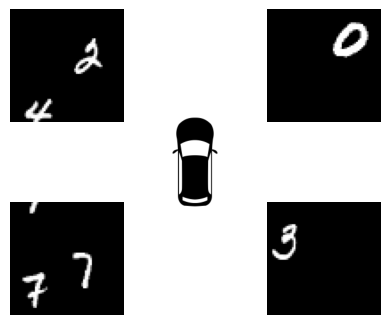
\includegraphics[width=0.33\textwidth]{figures/figure_methods_dataset_image_view_bev.png}
    \caption{Bird Eye View (BEV) of the frame raster divided into grid.}
    \label{fig:figure_methods_dataset_image_view_bev}
\end{figure}

Table~\ref{tab:results_multi_view} shows the inference results for multi-view setup we breakdown reasults by evaluation procedure. We train models under training schemas. 

% Results: https://docs.google.com/spreadsheets/d/1shITm2iWIKzAAlWpRwED-g1H6YurMJoJgxagRU2x6Gg/edit?gid=290835343#gid=290835343
% TODO Consider to reduce width of the table

\begin{table}[htb!]
    \centering
    \caption{Results for the "default" and "blind" experiments with sensor output shuffle. An asterisk (*) next to the model name indicates a training procedure with sensor output drops. The Average Displacement Error (ADE) measures the error for the second half of the sequence. The Final Displacement Error (FDE) evaluates the error for the last frame in the sequence.}
    \label{tab:results_multi_view}
    \begin{tblr}{
        hlines, vlines,
        colspec={l c c c c c c c c c},
        row{1}={font=\bfseries},
        row{2}={font=\bfseries},
    }
        \SetCell[r=2]{l}Model & \SetCell[c=2]{c}Default & & \SetCell[c=2]{c}Shuffle & & \SetCell[c=2]{c}Blind & & \SetCell[c=2]{c}Blind, Shuffle & & \SetCell[r=2]{l}{Params \\ (M)} \\
        & ADE & FDE & ADE & FDE & ADE & FDE & ADE & FDE &\\
        Perceiver & 0.760 & 0.753 & 23.701 & 23.759 & 17.952 & 25.568 & 25.559 & 24.696 & 1.2 \\
        Perceiver (s) & 0.823 & 0.814 & 0.812 & 0.799 & 13.644 & 20.124 & 13.670 & 20.080 & 1.2 \\
        Perceiver (d) & 0.881 & 0.937 & 4.043 & 4.345 & 1.471 & 2.093 & 5.648 & 7.341 & 1.2 \\
        Perceiver (d, s) & 1.073 & 1.152 & 0.956 & 1.022 & 1.729 & 2.345 & 1.632 & 2.287 & 1.2 \\
    \end{tblr}
\end{table}
